\begin{table}[H]
    {\renewcommand{\arraystretch}{1.2}%
    \setlength{\tabcolsep}{0.3em}%
\begin{tabular}{bababab}
\toprule

\rowcolor{white} \null &
\textbf{Synthetic$_{\mathbf{\mathcal{F}}}$} & \textbf{Synthetic$_{\mathbf{\mathcal{\beta}}}$} &
\textbf{Lehrpfad$_{\mathbf{\mathcal{F}}}$} & \textbf{Lehrpfad$_{\mathbf{\mathcal{\beta}}}$} &
\textbf{Office$_{\mathbf{\mathcal{F}}}$} & \textbf{Office$_{\mathbf{\mathcal{\beta}}}$} \\
\midrule

\rowcolor{lightgray}
\textbf{Keypoint Count} &
    \num{217505} & \num{44221} &
    \num{2168190} & \num{2198592} &
    \num{171000} & \num{171000} \\
\textbf{Correspondences} &
    \num{96371} & \num{26455} &
    \num{297949} & \num{222495} &
    \num{43037} & \num{36309} \\
\rowcolor{lightgray}
\textbf{True Positives} &
    \num{76603} & \num{22179} &
    \num{110339} & \num{35387} &
    \num{24025} & \num{15455} \\
\textbf{False Positives} &
    \num{59032} & \num{8865} &
    \num{648603} & \num{651091} &
    \num{48868} & \num{48697} \\
\rowcolor{lightgray}
\textbf{False Negatives} &
    \num{19768} & \num{4276} &
    \num{187610} & \num{187108} &
    \num{19012} & \num{20854} \\

\bottomrule
\end{tabular}

    }
    \caption{Performance indicators for the default configuration of the SIFT algorithm on the different datasets.}
\end{table}

Foo bar

\begin{figure}[H]
\begin{subfigure}[t]{0.45\linewidth}
    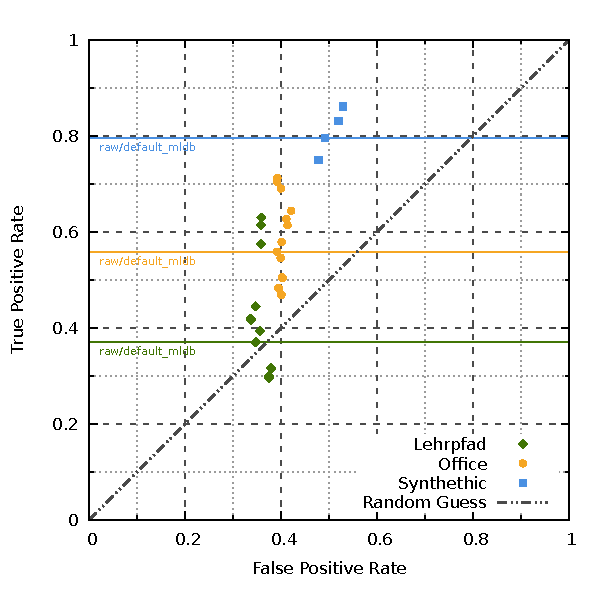
\includegraphics[width=\linewidth]{chapter06/results/AKAZE/flexion/roc.pdf}%
    \caption{Flexion Image ROC}
\end{subfigure}\quad
\begin{subfigure}[t]{0.45\linewidth}
    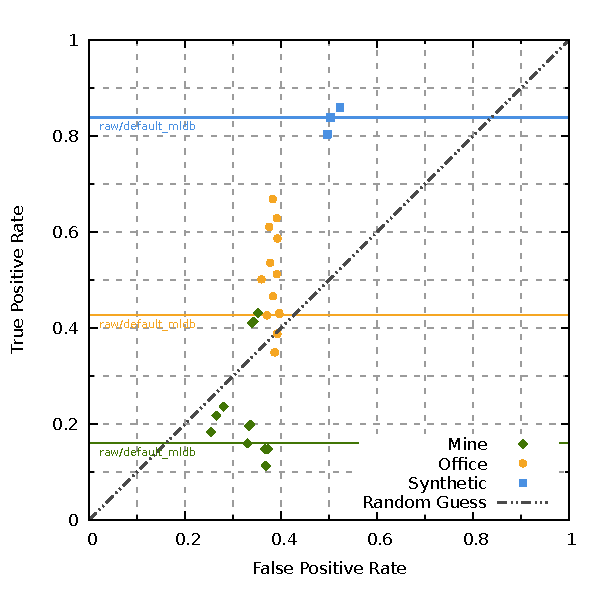
\includegraphics[width=\linewidth]{chapter06/results/AKAZE/bearing/roc.pdf}
    \caption{Bearing-Angle Image ROC}
\end{subfigure}
    \caption{AKAZE}
\end{figure}

\begin{figure}[H]
\begin{subfigure}[t]{0.45\linewidth}
    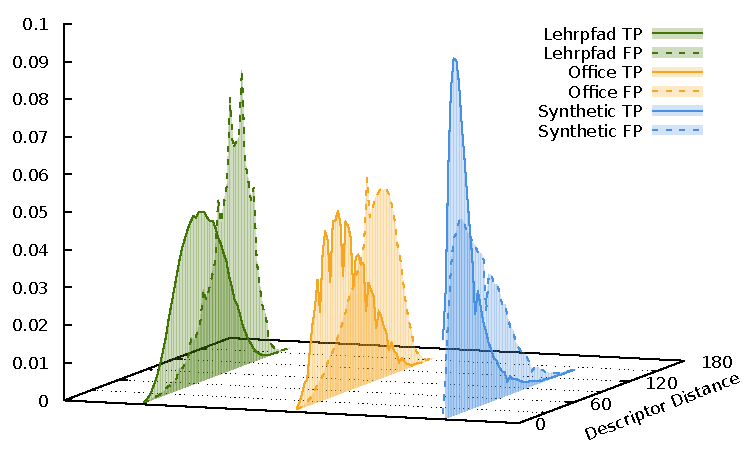
\includegraphics[width=\linewidth]{chapter06/results/AKAZE/flexion/descriptor_distances.pdf}%
    \caption{\gls{flexion-image} Descriptor Distances}
\end{subfigure}\quad
\begin{subfigure}[t]{0.45\linewidth}
    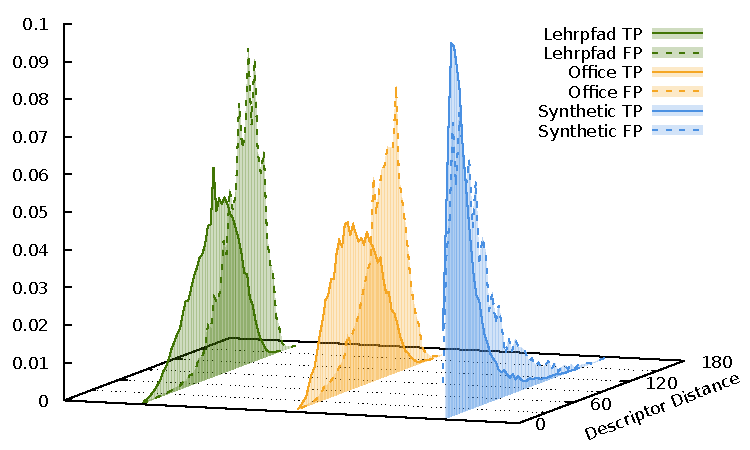
\includegraphics[width=\linewidth]{chapter06/results/AKAZE/bearing/descriptor_distances.pdf}%
    \caption{\gls{bearing-angle-image} Descriptors Distances}
\end{subfigure}
\end{figure}
